\documentclass[a4paper,12pt]{article}
%\documentclass[a4paper,10pt]{scrartcl}

\usepackage{scrextend}
\changefontsizes[14pt]{14pt}

\usepackage[T1]{fontenc}
\usepackage{lmodern}
\usepackage[utf8x]{inputenc}
\usepackage{graphicx}
\usepackage{tabularx}
\usepackage{multirow}
\usepackage{booktabs}
\usepackage{colortbl}
\usepackage[italian]{babel}
\usepackage[margin=2cm]{geometry}
\usepackage{color}
\definecolor{mygrey}{gray}{0.4}
\definecolor{light-blue}{rgb}{0.4,0.5,1}
\usepackage{booktabs}

%Header and footer of pages
\usepackage{fancyhdr}
\pagestyle{fancy}
\lhead{\textcolor{mygrey}{Emanuele Uliana, Gabriele Rufolo, Walter Rubino}}
\rhead{\textcolor{mygrey}{Design Document}}

%Set paragraphs indentation to 0 points
\setlength{\parindent}{0pt}

%Sections and subsections' style
\usepackage{titlesec} 
\titleformat{\section} {\color{blue}\normalfont\sffamily\Large\bfseries} {\color{blue}\thesection}{20pt}{} 
\usepackage{titlesec}
\titleformat{\subsection} {\color{light-blue}\normalfont\sffamily\large\bfseries\itshape} {\color{light-blue}\thesubsection}{18pt}{} 

%Document default font family
\renewcommand{\familydefault}{\sfdefault}
\renewcommand*\arraystretch{1.5}

\pdfinfo{%
  /Title    (SWIMv2 - Design Document)
  /Author  (Emanuele Uliana /and Gabriele Rufolo / and Walter Rubino)
  /Creator  (Emanuele Uliana /and Gabriele Rufolo / and Walter Rubino)
  /Producer (Emanuele Uliana /and Gabriele Rufolo / and Walter Rubino)
  /Subject  (Design Document)
  /Keywords ()

}

\begin{document}
\vspace*{\fill}
\begin{center}
{\fontsize{28}{10} \selectfont \textcolor{mygrey}{Progetto di Ingegneria del Software 2} \\[2\baselineskip]} {\fontsize{42}{10} \selectfont {\bfseries SWIMv2}} \\[4\baselineskip]

\includegraphics[scale=0.4]{polimi.png} \\[4\baselineskip]
{\fontsize{28}{10} \selectfont {\bfseries \textcolor{blue}{Design Document}} \\[2\baselineskip] A.A. 2012/2013}
\end{center}
\begin{flushleft}
{\fontsize{18}{10}
{\bfseries Autori}: \\ Emanuele Uliana (799256), Gabriele Rufolo (743695), Walter Rubino (742519) \\[1\baselineskip]
{\bfseries Docente}: \\ Prof.ssa Raffaela Mirandola
}
\end{flushleft}
\vspace*{\fill}
\begin{center}
Versione 1.0 del 22/12/2012 \\
\end{center}

\clearpage

	    \vspace*{\fill}
	\tableofcontents
	    \vspace*{\fill}

\clearpage

\section{Panoramica della piattaforma}
La piattaforma sviluppata ha il compito di promuovere, tramite l’utilizzo di una web application, la collaborazione e la condivisione di informazioni utili alla risoluzione di problemi tra gli utenti.\\[1\baselineskip]Nel dettaglio, il presente documento di Design definisce la struttura concettuale e funzionale fornendo una precisa descrizione delle guidelines che saranno seguite nello sviluppo e nel deployment dell’applicazione.\\[1\baselineskip]Il documento è inoltre conforme con le specifiche presenti nel RASD.\\[1\baselineskip]Il sistema è utilizzato da tre categorie di utenti: gli ospiti, gli utenti registrati e gli amministratori. Tramite un sistema di autenticazione il sistema controlla chi può svolgere determinate azioni in base al proprio ruolo.\\[1\baselineskip]Per evitare l’accesso a servizi non consentiti si è deciso di utilizzare il Role-Based Access Control. Con tale sistema di autenticazione si consentirà di usufruire solamente dei servizi specifici per il proprio ruolo.

\section{Descrizione del problema}
Il sistema è composto da varie pagine HTML ognuna delle quali fornisce uno specifico servizio al cliente. Ogni webpage include la tecnologia Javascript che consente non solo di migliorare l’interfaccia stessa della pagine ma permette anche di ottimizzare la facilità di navigazione.\\[1\baselineskip]Per sviluppare il sistema sono stati usati i seguenti tool:
\begin{itemize}
\item WaveMaker, per creare l’interfaccia grafica;
\item Eclipse Juno, per creare la logica di business;
\item Mysql, per gestire la base di dati.
\end{itemize}

La piattaforma SWIMv2 è un applicazione multi-tier composta dai seguenti livelli:
\begin{itemize}
\item Client tier: è composta dal client side dell’applicazione: si occupa di inviare le richieste al webserver tramite il browser. Include il codice Javascript e il codice HTML per la presentazione dei servizi.
\item Web tier: comprende le servlet per le risposte alle richieste Ajax e quindi con il client tier. Hanno anche il compito di gestire la sessione con gli utenti del sistema e di ricevere da quest’ultimi gli input inviati e di passarli quindi al business tier.
\item Business tier: gestisce la logica di sistema
\item Data tier: comprende la base di dati della quale si servirà il business tier. Tale base dati comprenderà tutti i dati e tutte le informazioni del sistema.
\end{itemize}

\subsection{Sottosistemi}
Sistemi che compongono l’applicazione: a noi servirà il login, i sottosistemi di ospite, utente registrato, amministratore e l’archiviazione dei messaggi, discussioni, registrazioni ecc.
\begin{itemize}
\item Login: sottosistema che si occupa della gestione dell’accesso al sistema, in base alla tipologia dell’utente seleziona il sottosistema di utilizzo; 
\item Archivio: sottosistema che si occupa della gestione degli accessi e degli utilizzi del DBMS del sistema; 
\item Ospite: gestisce il sistema con le ovvie restrizioni imposte dallo stato anonimo dell’utente ospite (impossibilità di replicare ai messaggi, inviare feedback…)
\item Utente registrato: questo sottosistema gestisce tutte le azioni dell’utente autenticato, i suoi permessi e le informazioni del suo profilo
\item Amministratore: gestisce sia tutte azioni esclusive dell’amministratore (come l’accettazione di nuove abilità) che quelle comuni all’utente registrato (come l’invio di messaggi)
\end{itemize}

L’esistenza dei sottosistemi dell’utenza di SWIM è giustificata dalla loro diversa interazione con l’archivio.\\[1\baselineskip]Gli amministratori potranno modificare le tabelle all’interno del DBMS, gli utenti registrati interagiranno con l’archiviazione dei messaggi e infine gli ospiti potranno visualizzare il contenuto di una parte dei dati senza poter apportare nessuna modifica.\\[1\baselineskip]Per gestire tale meccanismo abbiamo scelto una soluzione che prevede di sfruttare la logica dell’applicazione, essa sarà in un certo senso intelligente e secondo l’appartenenza di classe renderà possibili le corrispettive interazioni con il database.

\clearpage

\section{Design del Database}
\subsection{Modello concettuale}
Lo schema concettuale del Database in oggetto è stato modellato con un diagramma ER riportante le varie entità, i loro attributi e le relazioni presenti.\\
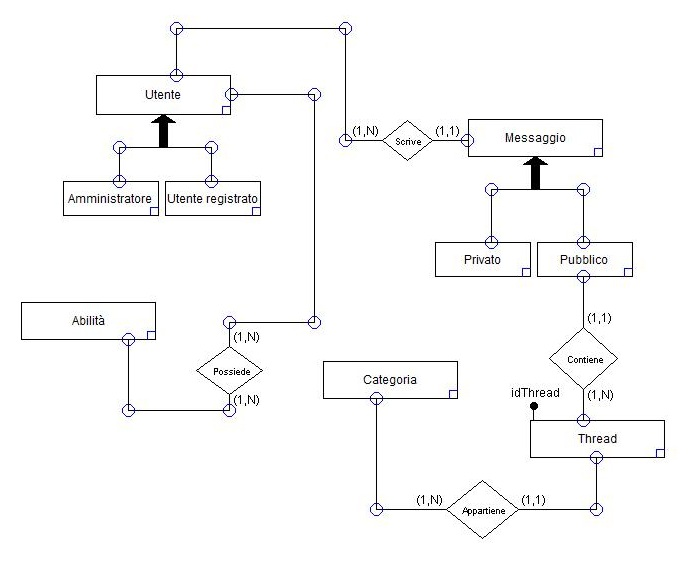
\includegraphics[scale=0.751]{modelloER.png}

\subsection{Modello logico}
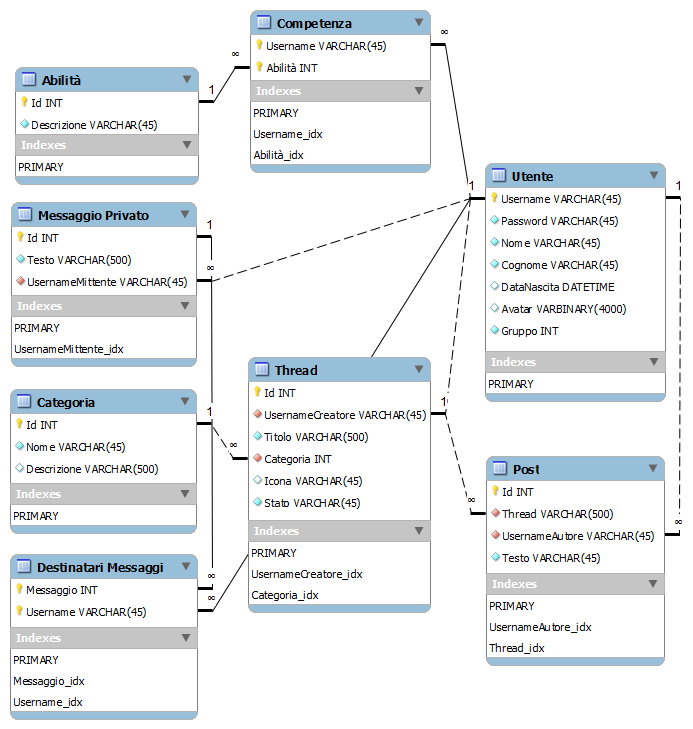
\includegraphics[scale=0.75]{ERMSWB.png}
Utente (\underline{Username}, Password, Nome, Cognome, DataNascita, Avatar,  Gruppo);\\
Competenza (\underline{Username}, \underline{Abilità});\\
Abilità (\underline{Id}, Descrizione);\\
MessaggioPrivato (\underline{Id}, Testo, UsernameMittente);\\
DestinatariMessaggio (\underline{Messaggio}, \underline{Username});\\
Post (\underline{Id}, Thread, UsernameAutore, Testo);\\
Thread (\underline{Id}, UsernameCreatore, Titolo, Categoria, Icona, Stato);\\
Categoria (\underline{Id}, Nome, Descrizione);\\

\end{document}